\section{Introduction}

Three branches of number theory: Elementary, Analytic, Algebraic, (Probabilistic)

Connections to other subjects: Discrete mathematics, physics, etc.

\subsection{Twin Primes}

Primes often appear in paris: 3 and 5, 5 and 7, 11 and 13.

\begin{definition}[Twin Primes]
    If $p$ and $p+2$ are primes, then we call them \textit{\textbf{twin primes}}.
\end{definition}

A famous conjecture is that there exits infinitely many primes.

\begin{conjecture}
    There exists infinitely many twin primes.
\end{conjecture}

A follow-up question to this conjecture is: Does the distance between consecutive primes become arbirarily large.

Let $\pi(x)$ denote the number of primes $\leq x$. For example, $\pi(6)=3$ because there are 3 primes, namely 2, 3, 5, less than or equal to 6. To answer this question, we would like to bound the number of primes less than or equal to $x$ as $x$ grows.

\begin{theorem}[Prime Number Theorem]
    As $x \to \infty$, $\pi(x) \sim \frac{x}{\log x}$.
\end{theorem}

This was first proved by Hadamard and de la Vall\'ee-Poussin in 1869. A slightly better bound uses the notion of a \textit{\textbf{logarithmic integral}}
$$
\mathrm{li}(x) = \int_2^x \frac{dt}{\log t} \sim \frac{x}{\log x}
$$
and
$$
\pi(x) = \mathrm{li}(x) + \underbrace{\Delta(x)}_{\text{error term}}
$$
Next, we bound the error term.

\begin{definition}[Big-O]
    We say that $f(x) = O(g(x))$ as $x \to \infty$ if there exists some constant $c > 0$ such that $|f(x)| \leq c|g(x)|$ for sufficiently large $x$.
\end{definition}

The Big-O notation is useful in number theory because it allows us to bound terms that we don't know the exact value of (for example, some error terms). The best known bound on $\pi(x)$ using big-O notation is
$$
\pi(x) = \mathrm{li}(x) + O\left( xe^{\frac{\log^{1/5}x}{(\log(\log(x)))^{1/5}}} \right) 
$$

It is also conjectured that $pi(x) = \mathrm{li}(x) + O(\sqrt{x} \log^2 x)$.

\section{Riemann Hypothesis}
Recall that the geometric series $\sum_{n=1}^\infty 1/n^x$ converges for $x > 1$. Similarly, $\sum_{n=1}^\infty 1/n^z$ converges for $\mathrm{Re}\; z > 1$.

We can generalize this for the Riemann zeta function.

\begin{theorem}
    $$
    \sum_{n=0}z^n = \frac{1}{1-z}
    $$
    when $|z| < 1$.

    The series $\sum_{n=0}z^n = \frac{1}{1-z}$ is also called the \textit{\textbf{Riemann zeta function}}, denote $\zeta(z)$. So this can be equivalently stated as: $\zeta(z)$ has an \textbf{analytic continuation} to the entire complex plane.
\end{theorem}
\begin{conjecture}[Riemann Hypothesis]
    All non-trivial zeros of the Riemann zeta function are on $\mathrm{Re}\; z = 1/2$.
\end{conjecture}

Pictorially, the Riemann hypothesis can be visualized using the diagram below.

\begin{figure}[htbp]
    \centering
    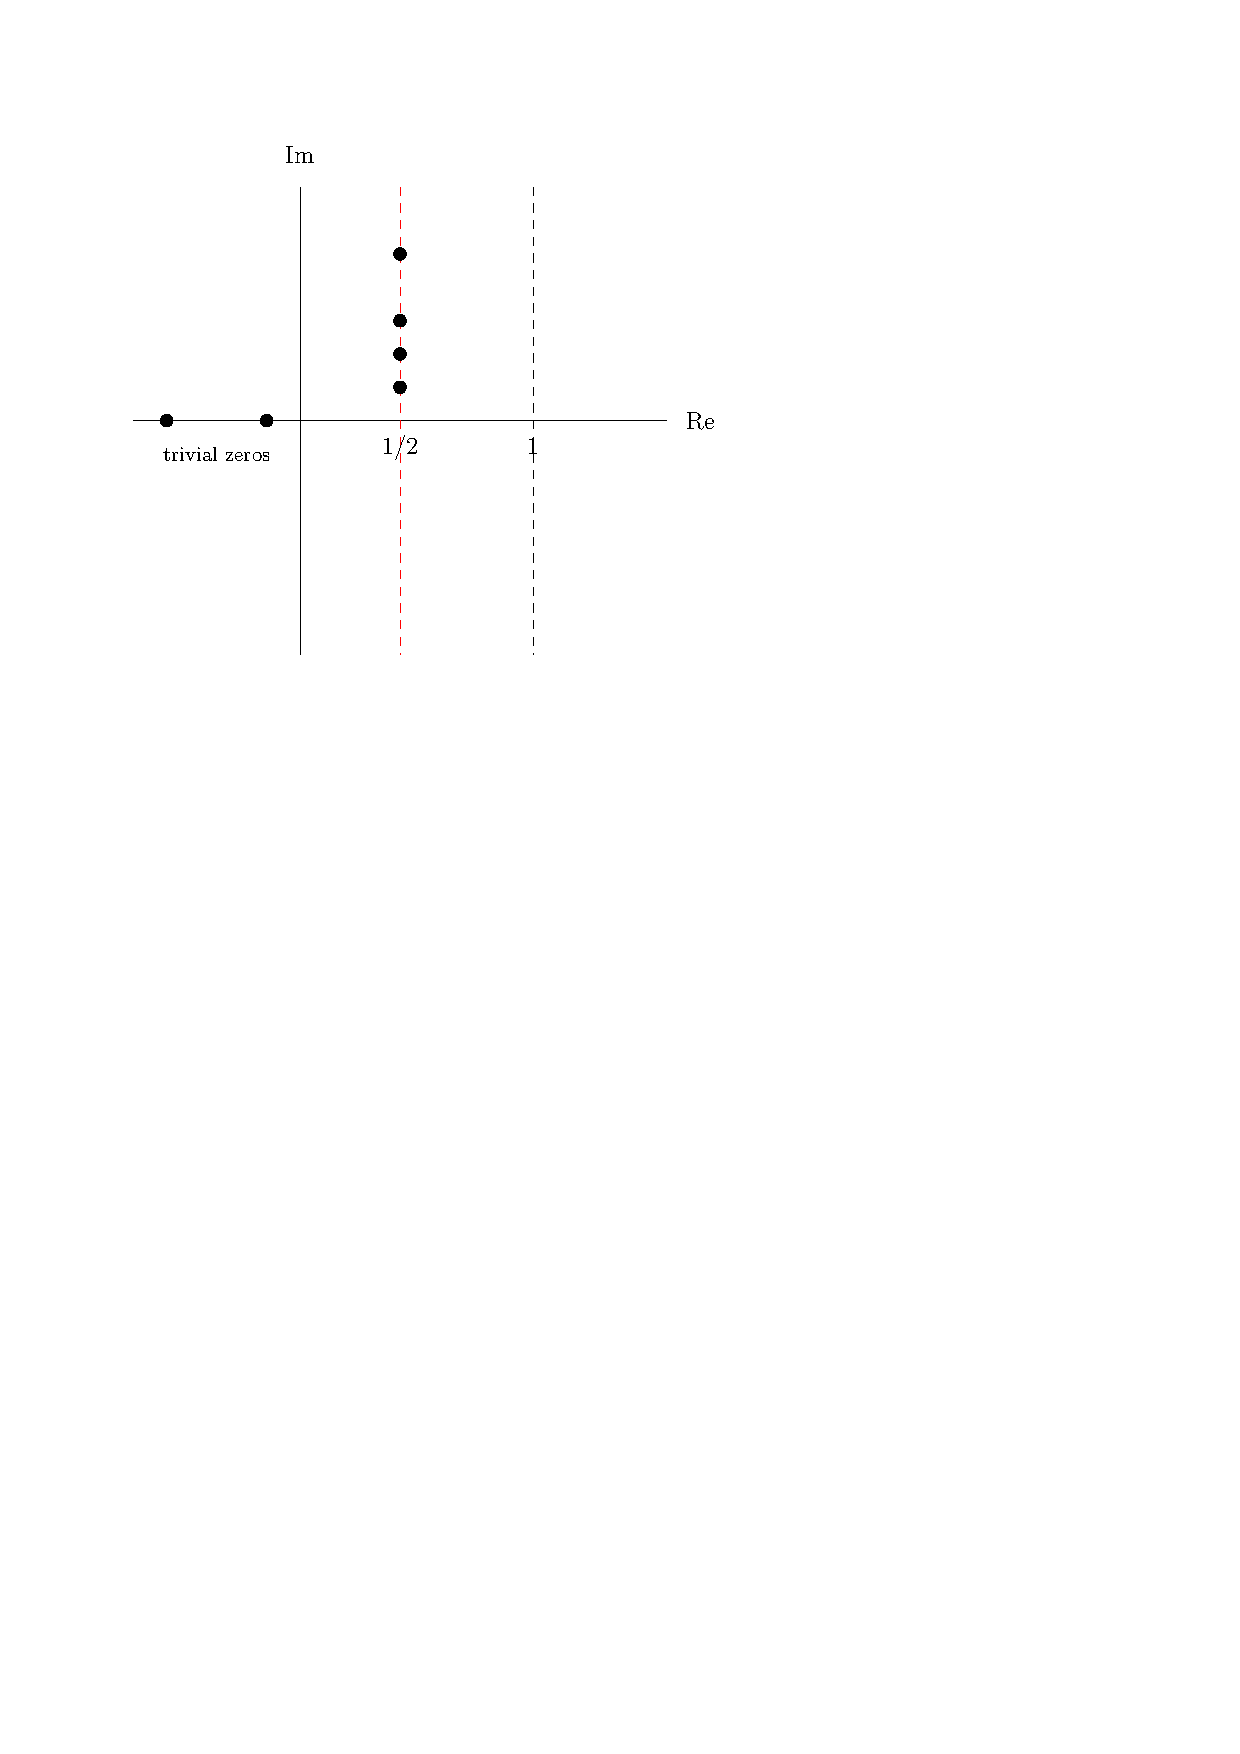
\includegraphics[width=.5\linewidth]{figures/riemann-hypothesis.pdf} 
    \caption{The non-trivial zeros of $\zeta(z)$ on a complex plane.}
    \label{fig:riemann-hypothesis}
\end{figure}

\section{Sum of Two Squares}

Recall that $a \equiv b \mod c$ if and only if $c \divides (a-b)$. 

If $p \equiv 1 \mod 4$, we will show that $p = a^2 + b^2$ for some integers $a$ and $b$. Such pair of $a,b$ where $a,b \in \Z$ is called a \textit{\textbf{lattice point}}.

\begin{theorem}[Fermat's theorem on sum of two squares]
    An odd prime $p$ can be expressed as $p = x^2 + y^2$ with integers $x$ and $y$ if and only if $p \equiv 1 \mod 4$.
\end{theorem}

Let $r_2(n)$ denote the number of representations of $n$ as a sum of two squares. We would like to study the behavior of $\sum_{n \leq x} r_2(n)$.

We start with \textbf{Gauss's attempt} in trying to bound $\sum_{n \leq x} r_2(n)$. As we can see, each lattice point can be represented as the coordinate $(m,n)$ of a point on a plane. If we draw a circle with radius $r$, then all lattice points within the circle have the property
$$
m^2 + n^2 \leq r^2
$$
Then, the problem of bounding $\sum_{n\leq x}r_2(n)$ for some $x$ is the same as finding the number of lattice points within the circle centered at $(0,0)$ with radius $\sqrt{x}$. Because of this, the problem is also known as \textit{\textbf{Gauss circle problem}}.

\begin{figure}[htbp]
    \centering
    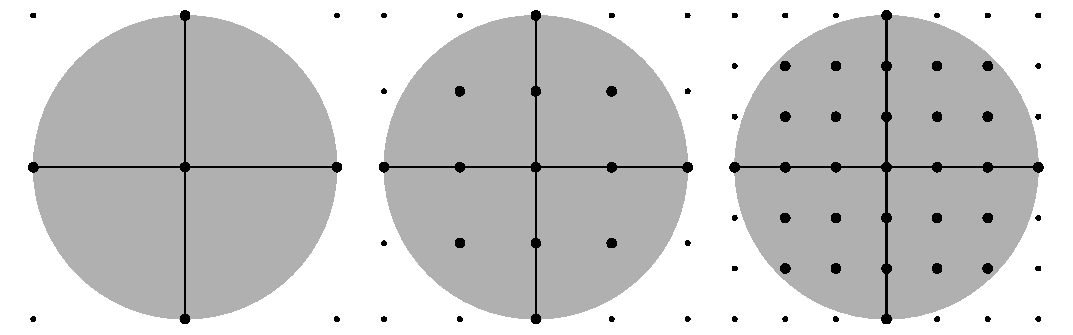
\includegraphics[width=0.5\linewidth]{figures/GausssCircleProblem.pdf}
    \caption{Gauss's circle problem}
    \label{fig:gauss-circle-prob}
\end{figure}

\begin{theorem}[Gauss's solution]
    $$
    \sum_{n \leq x} r_2(n) = \pi x + O(\sqrt{x}) = \pi x + \underbrace{E(x)}_{\text{error term}}
    $$
    So, $E(x) \in O(x^{1/2})$.
\end{theorem}

\begin{proof}
    We associate each representation of a number as two squares with a square on the plane, enclosed within the circle of radius $\sqrt{x}$.

    Then, the number of such lattice points is bounded above by the area of the larger circle and bounded below by the smaller circle.
    $$
    \pi(\sqrt{x} - 1)^2 \leq \sum_{n \leq x}r_2(n) \leq \pi(\sqrt{x} + 1)^2
    $$
    \begin{figure}[htbp]
        \centering
        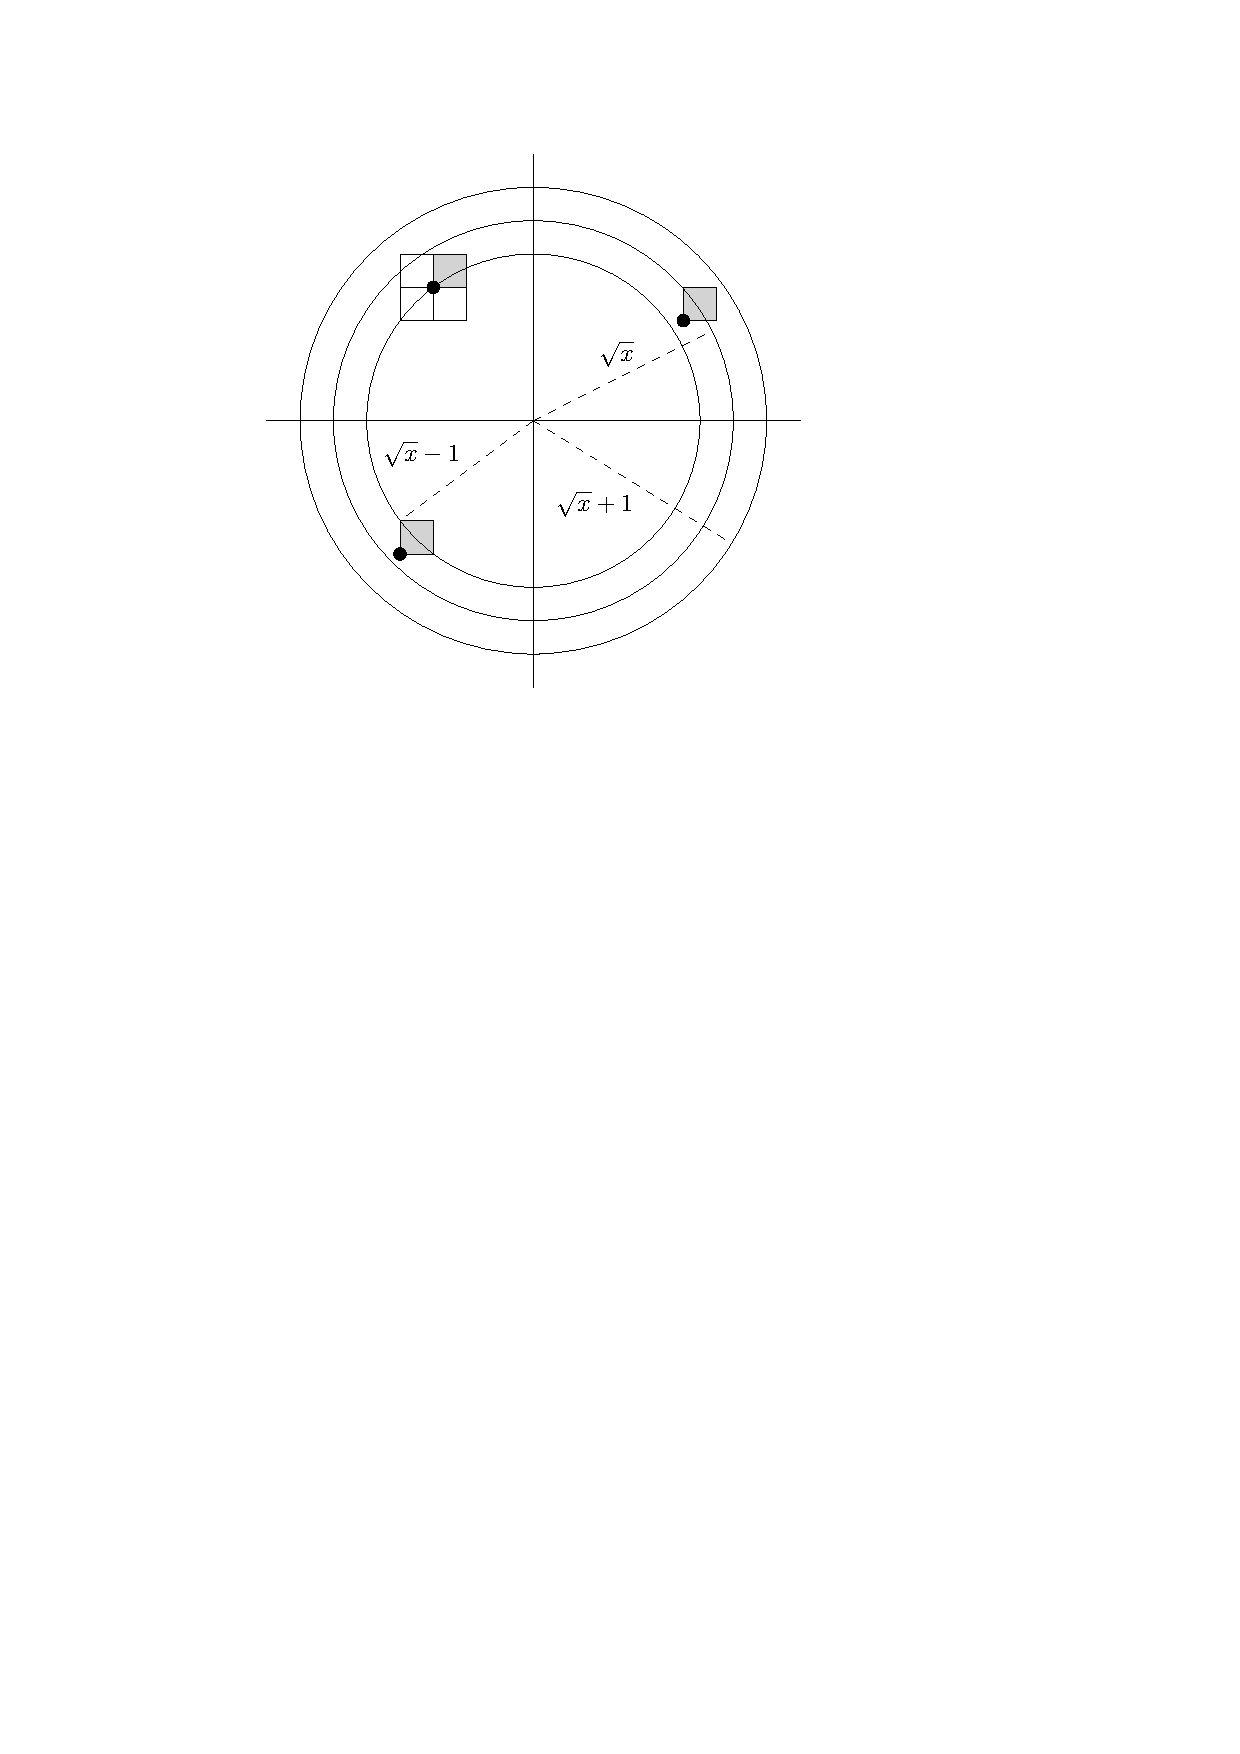
\includegraphics[width=.4\linewidth]{figures/gauss-circle-area.pdf}
        \caption{Using area to bound the number lattice points.}
        \label{fig:gauss-circle-area}
    \end{figure} 
    We can further rearrange this to get
    $$
    \pi(x - 2\sqrt{x+1}) \leq \sum_{n \leq x} r_2(n) \leq \pi(x + 2\sqrt{x} + 1)
    $$
    Then, $\sum_{n\leq x}r_2(n) = \pi x + O(\sqrt{x})$. 
\end{proof}

Over the years, there have been numerous improvements on bounding the error term.

\begin{theorem}[Sierpinski 1906]
    $$
    \sum_{n \leq x} r_2(n) = \pi x + O(x^{1/3})
    $$
\end{theorem}

\section{Integer Partition}

Next, we will consider the integer partition. A \textit{\textbf{partition}} of an integer $n \in \Z^+$ is one way of representing $n$ as a sum of \textbf{more than one} (possibly repeating) integers.

We define $P(n)$ to be the number of ways of writing $n \in \Z^+$ as a sum of positive integers (ways to partition $n$).

For example, $P(4) = 5$ because $4 = 3+1 = 2+2 = 2+1+1 = 1+1+1+1$. Note that $4$ itself does not count since we need at least 2 integers for it to be a valid partition.

\begin{conjecture}[Ramanujan's Conjecture on Integer Partition]
    $P(5n + 4) \equiv 0 \mod 5$, $P(7n + 5) \equiv 0 \mod 7$, $P(11n + 6) \equiv 0 \mod 11$.
\end{conjecture}